\newpage
\section[Day 5: Metric Spaces and Set Types]{Metric Spaces}

\subsection{ Set of Sets } 

{ \color{blue} Definition 5.1.1: Union and Intersection } 

	\begin{adjustbox}{minipage=14cm, right}
		Let sets $\Omega$,B be such that for each x $\in$ $\Omega$,
		there is an associated E$_x$ $\subset$ B.
		\begin{itemize}[leftmargin=1cm, itemsep=0.4em]
			\item E = $\cup_{x=1}^{n}$ E$_x$ only if for every x $\in$ E, x $\in$ E$_x$ for
				at least one x $\in$ $\Omega$.

			\item P = $\cap_{x=1}^{n}$ E$_x$ only if for every x $\in$ P, x $\in$ E$_x$ for
				all x $\in$ $\Omega$.
		\end{itemize}
		with properties:
	\end{adjustbox}

	\begin{enumerate}[label=(\alph*), leftmargin=2cm, itemsep=0.4em]
		\item A $\cup_{}^{}$ B = B $\cup_{}^{}$ A
			\hspace{4cm} A $\cap_{}^{}$ B = B $\cap_{}^{}$ A

		\item (A $\cup_{}^{}$ B) $\cup_{}^{}$ C = A $\cup_{}^{}$ (B $\cup_{}^{}$ C)
			\hspace{1.6cm} (A $\cap_{}^{}$ B) $\cap_{}^{}$ C = A $\cap_{}^{}$ (B $\cap_{}^{}$ C)

		\item A $\subset$ A $\cup_{}^{}$ B
			\hspace{4.8cm} (A $\cap_{}^{}$ B) $\subset$ A

		\item If A $\subset$ B, then A $\cup_{}^{}$ B = B and A $\cap_{}^{}$ B = A

			{ \color{magenta} \underline{Proof} } 
			
				If x $\in$ A $\cup_{}^{}$ B, then x $\in$ A or/and x $\in$ B.
				\begin{itemize}[leftmargin=1cm, itemsep=0.4em]
					\item If x $\in$ A, since A $\subset$ B, then x $\in$ B.
						Then, (A $\cup_{}^{}$ B) $\subset$ B.

					\item If x $\in$ B, then immediately (A $\cup_{}^{}$ B) $\subset$ B.
				\end{itemize}
				If x $\in$ B, then x $\in$ A $\cup_{}^{}$ B so B $\subset$ (A $\cup_{}^{}$ B).
				Thus, A $\cup_{}^{}$ B = B.

				\vspace{0.5cm}

				If x $\in$ A $\cap_{}^{}$ B, then x $\in$ A and x $\in$ B.
				Thus, (A $\cap_{}^{}$ B) $\subset$ A.

				If x $\in$ A, since A $\subset$ B, then x $\in$ B so x $\in$ A $\cap_{}^{}$ B.
				Thus, A $\subset$ (A $\cap_{}^{}$ B).

				Thus, A $\cap_{}^{}$ B = A.

		\item A $\cap_{}^{}$ (B $\cup_{}^{}$ C) = (A $\cap_{}^{}$ B) $\cup_{}^{}$ (A $\cap_{}^{}$ C)

			{ \color{magenta} \underline{Proof} } 
			
				If x $\in$ A $\cap_{}^{}$ (B $\cup_{}^{}$ C), then x $\in$ A
				and (x $\in$ B or/and x $\in$ C).
				\begin{itemize}[leftmargin=1cm, itemsep=0.4em]
					\item If x $\in$ B, then x $\in$ (A $\cap_{}^{}$ B) so
						x $\in$ (A $\cap_{}^{}$ B) $\cup_{}^{}$ (A $\cap_{}^{}$ C).

					\item If x $\in$ C, then x $\in$ (A $\cap_{}^{}$ C) so
						x $\in$ (A $\cap_{}^{}$ B) $\cup_{}^{}$ (A $\cap_{}^{}$ C).
				\end{itemize}
				Thus, A $\cap_{}^{}$ (B $\cup_{}^{}$ C)
				$\subset$ (A $\cap_{}^{}$ B) $\cup_{}^{}$ (A $\cap_{}^{}$ C).
				
				If x $\in$ (A $\cap_{}^{}$ B) $\cup_{}^{}$ (A $\cap_{}^{}$ C),
				then x $\in$ A and (x $\in$ B or/and x $\in$ C).

				Thus, (A $\cap_{}^{}$ B) $\cup_{}^{}$ (A $\cap_{}^{}$ C)
				$\subset$ A $\cap_{}^{}$ (B $\cup_{}^{}$ C).

				Thus, A $\cap_{}^{}$ (B $\cup_{}^{}$ C)
				= (A $\cap_{}^{}$ B) $\cup_{}^{}$ (A $\cap_{}^{}$ C).

		\item A $\cup_{}^{}$ (B $\cap_{}^{}$ C) = (A $\cup_{}^{}$ B) $\cap_{}^{}$ (A $\cup_{}^{}$ C)

			{ \color{magenta} \underline{Proof} } 
			
			If x $\in$ A $\cup_{}^{}$ (B $\cap_{}^{}$ C), then
			x $\in$ A or/and (x $\in$ B and x $\in$ C).
			\begin{itemize}[leftmargin=1cm, itemsep=0.4em]
				\item If x $\in$ A, then x $\in$ (A $\cup_{}^{}$ B)
					and x $\in$ (A $\cup_{}^{}$ C)
					so A $\cup_{}^{}$ (B $\cap_{}^{}$ C) $\subset$
					(A $\cup_{}^{}$ B) $\cap_{}^{}$ (A $\cup_{}^{}$ C).

				\item If x $\in$ B,C, then x $\in$ (A $\cup_{}^{}$ B)
					and x $\in$ (A $\cup_{}^{}$ C)
					so A $\cup_{}^{}$ (B $\cap_{}^{}$ C) $\subset$
					(A $\cup_{}^{}$ B) $\cap_{}^{}$ (A $\cup_{}^{}$ C).
			\end{itemize}
			If x $\in$ (A $\cup_{}^{}$ B) $\cap_{}^{}$ (A $\cup_{}^{}$ C), then
			x $\in$ A or/and (x $\in$ B and x $\in$ C).

			Thus, (A $\cup_{}^{}$ B) $\cap_{}^{}$ (A $\cup_{}^{}$ C)
			$\subset$ A $\cup_{}^{}$ (B $\cap_{}^{}$ C).

			Thus, A $\cup_{}^{}$ (B $\cap_{}^{}$ C)
			= (A $\cup_{}^{}$ B) $\cap_{}^{}$ (A $\cup_{}^{}$ C).
	\end{enumerate}

\newpage

{ \color{red} Theorem 5.1.2: Union of countably infinite sets is countably infinite } 

	\begin{adjustbox}{minipage=14cm, right}
		If $E_1, E_2, ... $ are countably infinite sets, then S = $\cup_{n=1}^{\infty}$ $E_n$
		is countably infinite.
	\end{adjustbox}

{ \color{magenta} \underline{Proof} } 
	
	For each $E_n$, there is a sequence \{ $x_{n1}$, $x_{n2}$, ... \}.
	Then construct an array as such:

	$ \hspace{1cm}
	\left(
	\begin{array}{cccc}
		x_{11} & x_{12} & x_{13} & ... \\
		x_{21} & x_{22} & x_{23} & ... \\
		x_{31} & x_{32} & x_{33} & ... \\
		\vdots & \vdots & \vdots & \ddots \\
	\end{array}
	\right)
	$
		
	Take elements diagonally, then sequence S$^*$ =
	\{ $x_{11} \ ; \ x_{21}, x_{12} \ ; \ x_{31}, x_{32}, x_{33} \ ; \ ... $ \}.
		
	\begin{adjustbox}{minipage=15cm, right}
		Since S$^*$ $\sim$ S so S is at most countable and S is infinite since
		$E_1, E_2, ...$ are infinite, then S cannot be finite and thus, countably infinite.
	\end{adjustbox}

{ \color{magenta} \underline{Alternative Proof} } 

	For each $E_n$, let set $\widetilde{E_n}$ = $E_n$ - $\cup_{m=1}^{\infty}$ $E_m$ where
	m $\neq$ n. Thus, S = $\cup_{n=1}^{\infty}$ $\widetilde{E_n}$.

	Since each $E_n$ is countably infinite, there exists a 1-1 mapping
	$\delta_n$: $E_n$ $\rightarrow$ $\mathbb{Z}_+$.

	Thus, for each $\widetilde{E_n}$, there is a 1-1 mapping
	$\delta_n$: $\widetilde{E_n}$ $\rightarrow$ A $\subset$ $\mathbb{Z}_+$.

	Let $p_1, p_2, ... $ be distinct primes.

	Since for s $\in$ S, there exists a unique $\widetilde{E_i}$ such that
	s $\in$ $\widetilde{E_i}$, then let f(s) = $p_1^{\delta_1(s)} p_2^{\delta_2(s)}...$
	where $p_k^{\delta_k(s)}$ = 1 if k $\neq$ i.

	Then, by the Fundamental theorem of arithmetic, f maps s to a unique z $\in$ $\mathbb{Z}_+$
	and thus, f is a 1-1 function so S is at most countable.

	Since any $E_n$ $\subset$ S is countably infinite, then S cannot be finite
	and thus, S is countably infinite.

\begin{figure}[h]
	\centering
	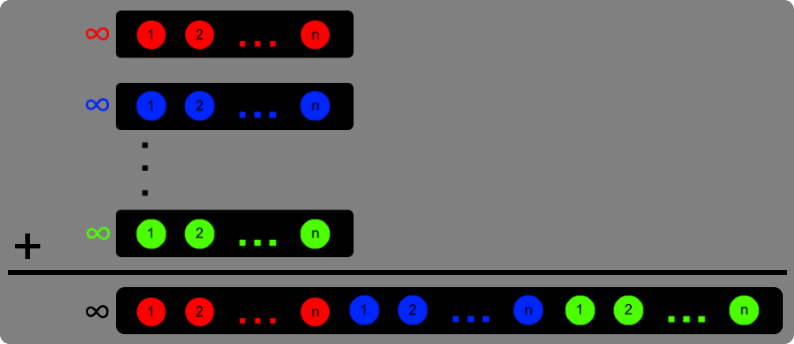
\includegraphics[scale=0.5]{Images/5.1.2.png}
\end{figure}

{ \color{red} Theorem 5.1.3: The set of countable n-tuples are countable } 

	\begin{adjustbox}{minipage=14cm, right}
		Let A be a countably infinite set and B$_n$ be the set of all
		n-tuples ($a_1$,...,$a_n$) where $a_k$ $\in$ A.
		Then $B_n$ is countably infinite.
	\end{adjustbox}

{ \color{magenta} \underline{Proof} } 
	
	The base case $B_1$ is countably infinite since $B_1$ = A.

	Suppose $B_{n-1}$ is countably infinite. Then for every x $\in$ B:

	\qquad x = (b,a) \qquad \qquad b $\in$ $B_{n-1}$ and a $\in$ A

	Since for every fixed b, (b,a) $\sim$ A and thus, countably infinite.

	Since B is a set of countably infinite sets, then $B_{n}$
	is countably infinite. \\

{ \color{blue} Definition 5.1.4: $\mathbb{Q}$ is countably infinite } 

	\begin{adjustbox}{minipage=14cm, right}
		The set of rational numbers, $\mathbb{Q}$, is countably infinite.
	\end{adjustbox}

{ \color{magenta} \underline{Proof} } 
	
	Since elements of $\mathbb{Q}$ are of form $\frac{a}{b}$ which is a
	2-tuple, then by the {\color{red} theorem 5.1.3}, $\mathbb{Q}$ is countably infinite.

{ \color{magenta} \underline{Alternative Proof} } 
	
	For every x $\in$ $\mathbb{Q}$, let x = $(-1)^i$ $\frac{p}{q}$ where p,q $\in$ $\mathbb{Z}_+$.

	Let f(x) = $2^i$ $3^p$ $5^q$. Then by the Fundamental theorem of arithmetic,
	f is a 1-1 mapping of x to E $\subset$ $\mathbb{Z}_+$.

	Thus, $\mathbb{Q}$ is at most countable, but since p,q $\in$ $\mathbb{Z}_+$,
	then $\mathbb{Q}$ cannot be finite and thus, is countably infinite. \\

{ \color{purple} Example 5.1.5: Sequences of 0 and 1 are uncountable } 

	\begin{adjustbox}{minipage=14cm, right}
		Let A be the set of all sequences whose elements are digits 0 and 1.
		Then A is uncountable.
	\end{adjustbox}

{ \color{magenta} \underline{Proof: Cantor's Diagonalization Proof} } 

	Let set E be a countably infinite subset of A which consist of sequences $s_1,s_2,...$.

	Then construct a sequence s as follows:

	\qquad If the n-th digit in $s_n$ is 1, then let the n-th digit of s be 0
	and vice versa.

	Thus. s differs from every $s_n$ $\in$ E so s $\not \in$ E.

	But, s $\in$ A so E is a proper subset of A.

	Thus, every countably infinite subset of A is a proper subset of A.

	If A is countably infinite, then A is a proper subset of A which
	is a contradiction.





\subsection{ Metric Spaces }

{ \color{blue} Definition 5.2.1: Metric Spaces } 

	\begin{adjustbox}{minipage=14cm, right}
		A set X is a metric space if for ant p,q $\in$ X, there is an associated d(p,q) $\in$
		$\mathbb{R}$ such that:	
		\begin{itemize}[leftmargin=1cm, itemsep=0.4em]
			\item d(p,q) $>$ 0 \qquad \qquad if p $\neq$ q
			
			\item d(p,q) = 0 if and only if p = q
			
			\item {\color{lblue} Symmetry}:
				d(p,q) = d(q,p)
			
			\item {\color{lblue} Triangle Inequality}:
				d(p,q) $\leq$ d(p,r) + d(r,q) \qquad \qquad for any r $\in$ $\mathbb{R}$.
		\end{itemize}

		For euclidean spaces $\mathbb{R}^k$, d(x,y) = $| x - y |$ where x,y $\in$ $\mathbb{R}^k$. \\
	\end{adjustbox}

{ \color{blue} Definition 5.2.2: Types of points and sets } 
	\begin{enumerate}[label=(\alph*), leftmargin=2cm, itemsep=0.4em]
		\item {\color{lblue} Neighborhood}

			\qquad For p $\in$ $\mathbb{R}^k$ and r $>$ 0, N$_r(p)$ is the set of all q
			such that d(q,p) $<$ r

			\begin{figure}[h]
				\centering
				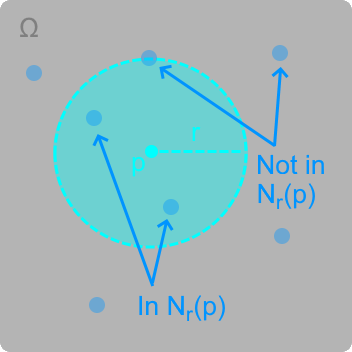
\includegraphics[scale=0.45]{Images/5.2.2a.png}
			\end{figure}

		\item {\color{lblue} Limit Points and Closed Sets}

			\qquad Closed set E contains all p where every N$_r(p)$ contains
			a q $\neq$ p $\in$ E
			\begin{itemize}[leftmargin=1cm, itemsep=0.4em]
				\item Limit Points 

					\qquad For point p $\in$ X, every N$_r(p)$ contains a
					q $\neq$ p $\in$ E
				
				\item Isolated Points

					\qquad If p $\in$ E is not a limit point of E

				\item Closed

					\qquad If every limit point p of E is a p $\in$ E
			\end{itemize}

			\begin{figure}[h]
				\centering
				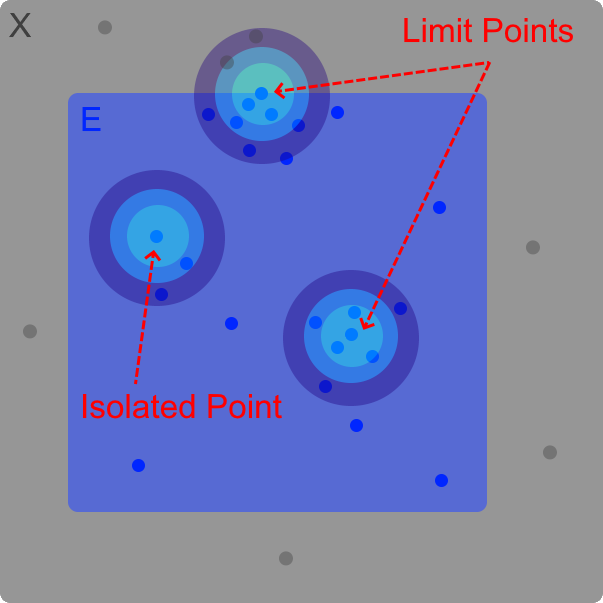
\includegraphics[scale=0.3]{Images/5.2.2b.png}
			\end{figure}

		\item {\color{lblue} Interior Points and Open Sets}

			\qquad Open set E contains all its p which has a N$_r(p)$ $\subset$ E
			\begin{itemize}[leftmargin=1cm, itemsep=0.4em]
				\item Interior Point

					\qquad For p $\in$ X, there is a N$_r(p)$ $\subset$ E

				\item Open

					\qquad If every p $\in$ E is an interior point of E
			\end{itemize}

			\begin{figure}[h]
				\centering
				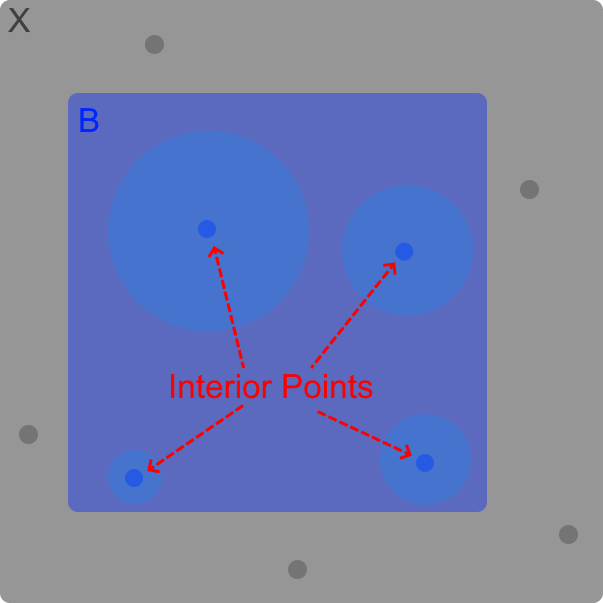
\includegraphics[scale=0.3]{Images/5.2.2c.png}
			\end{figure}

		\item {\color{lblue} More about Sets}
			\begin{itemize}[leftmargin=1cm, itemsep=0.4em]
				\item Bounded

					\qquad If there is M $\in$ $\mathbb{R}$ , q $\in$ X such that d(p,q) $<$ M
					for all p $\in$ E

				\item Complement

					\qquad From E, E$^\text{c}$ is the set of all p $\in$ X such that p $\not \in$ E

				\item Perfect

					\qquad If E is closed and if every p $\in$ E is a limit point of E

				\item Dense

					\qquad If every p $\in$ X is a limit point of E or/and p $\in$ E \\
			\end{itemize}
	\end{enumerate}

\newpage

{ \color{red} Theorem 5.2.3: N$_r(p)$ is open } 

	\begin{adjustbox}{minipage=14cm, right}
		Every neighborhood is an open set.
	\end{adjustbox}

{ \color{magenta} \underline{Proof} } 
	
	Let q $\in$ N$_r(p)$. Then there is a h $>$ 0 $\in$ $\mathbb{R}$
	such that d(q,p) = r - h.

	Then for any s $\in$ N$_h(q)$:

	\qquad d(s,p) $\leq$  d(s,q) + d(q,p) = h + (r - h) = r

	Thus, for any q $\in$ N$_r(p)$, there exists a N$_h(q)$ $\subset$ N$_r(p)$.

\begin{figure}[h]
	\centering
	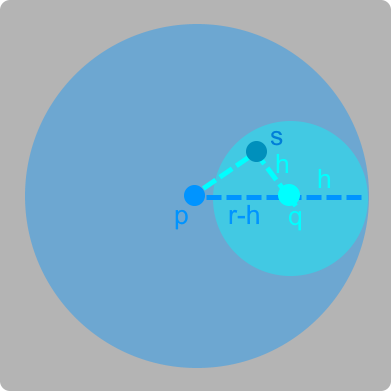
\includegraphics[scale=0.38]{Images/5.2.3.png}
\end{figure}

{ \color{red} Theorem 5.2.4: If a set has a limit point, there are infinite q
$\in$ E in N$_r(p)$ } 
	
	\begin{adjustbox}{minipage=14cm, right}
		If p is a limit point of set E, then every N$_r(p)$ contains infinitely many q $\in$ E.
	\end{adjustbox}

{ \color{magenta} \underline{Proof} } 
	
	Suppose there is N$_{r_1}(p)$ which contains finitely many q = \{ q$_1$, ... , q$_n$ \}.

	Let r = min$_{m \in [1,n]}$ d(p,q$_m$). Then N$_r(p)$ contains no q $\in$ E such that q $\not =$ p.

	So, p is not a limit point of E which is a contradiction since p is a limit point of E.

\begin{figure}[h]
	\centering
	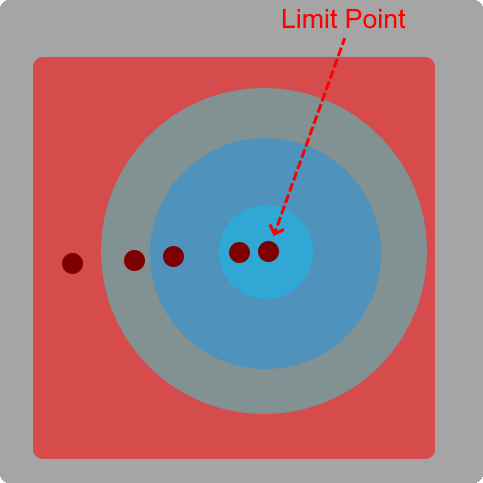
\includegraphics[scale=0.33]{Images/5.2.4.png}
\end{figure}

{ \color{orange} Corollary 5.2.5: Limit points do not exist in finite sets } 
	
	\begin{adjustbox}{minipage=14cm, right}
		A finite set has no limit points.
	\end{adjustbox}

{ \color{magenta} \underline{Proof} } 

	Let p be a limit point of finite set E. By {\color{red} theorem 5.2.4}, 
	then any N$_r(p)$ contain infinite q $\in$ E so E is an infinite set
	which is a contradiction since E is finite.

	So p cannot be limit point of E and thus, E has no limit points. \\

{ \color{red} Theorem 5.2.6: De Morgan's Laws } 
	
	\begin{adjustbox}{minipage=14cm, right}
		Let $E_1, E_2 , ... $ be a collection of sets. Then,
		($\cup_{}^{}$ $E_x$)$^\text{c}$ = $\cap_{}^{}$ ($E_x$$^\text{c}$).
	\end{adjustbox}

{ \color{magenta} \underline{Proof} } 
	
	If p $\in$ ($\cup_{}^{}$ $E_x$)$^\text{c}$, then p $\not \in$ ($\cup_{}^{}$ $E_x$).

	Thus, p $\not \in$ $E_x$ for any x so p $\in$ E$_x^\text{c}$ for all x.
	Thus, p $\in$ $\cap_{}^{}$ ($E_x^c$) so
	($\cup_{}^{}$ $E_x$)$^c$ $\subset$ $\cap_{}^{}$ ($E_x^c$).

	If p $\in$ $\cap_{}^{}$ ($E_x^c$), then p $\in$ $E_x^c$ for all x.
	
	Thus, p $\not \in$ $E_x$ for any x so p $\not \in$ $\cup_{}^{}$ $E_x$.
	Thus, p $\in$ ($\cup_{}^{}$ $E_x$)$^c$ so
	$\cap_{}^{}$ ($E_x^c$) $\subset$ ($\cup_{}^{}$ $E_x$)$^c$.

	Thus, ($\cup_{}^{}$ $E_x$)$^c$ = $\cap_{}^{}$ ($E_x^c$). \\

{ \color{red} Theorem 5.2.7: Open set $\rightarrow$ Closed complement } 

	\begin{adjustbox}{minipage=14cm, right}
		A set E is open if and only if E$^\text{c}$ is closed.
	\end{adjustbox}

{ \color{magenta} \underline{Proof} } 

	Suppose E is open. Let x be a limit point of E$^c$.

	Then for every r $>$ 0, N$_r(x)$ must contain a p $\in$ E$^c$ such that p $\neq$ x.

	Then, N$_r(x)$ $\not \subset$ E so x is not an interior point of E and
	thus, x $\not \in$ E so x $\in$ E$^c$.

	Since any limit point x of E$^c$ is a x $\in$ E$^c$, then E$^c$ is closed.

	\vspace{0.2cm}

	Suppose E$^c$ is closed. Let x $\in$ E.

	Since x $\not \in$ E, x is not a limit point of E.

	Then there exists a r $>$ 0 such that any p $\in$ N$_r(x)$ is not in E.

	Thus, every p $\in$ N$_r(x)$ is p $\in$ E so N$_r(x)$ $\subset$ E and thus,
	x is an interior point of E.

	Since any x $\in$ E is an interior point of E, then E is open. \\

{ \color{orange} Corollary 5.2.8: Closed set $\rightarrow$ Open complement } 

	\begin{adjustbox}{minipage=14cm, right}
		A set F is closed if only only if F$^\text{c}$ is open.
	\end{adjustbox}

{ \color{magenta} \underline{Proof} } 

	From {\color{red} theorem 5.2.7}, let E = F$^\text{c}$. \\

{ \color{red} Theorem 5.2.9: Union open $\rightarrow$ open and
Intersection closed $\rightarrow$ closed } 

	\begin{enumerate}[label=(\alph*), leftmargin=2cm, itemsep=0.4em]
		\item If $\{G_x\}$ is a finite or infinite collection of open sets,
		then $\cup$ $G_x$ is open.

			{ \color{magenta} \underline{Proof} }

				If p $\in$ $\cup$ $G_x$, then p $\in$ $G_x$ for at least one x.
				Let $\overline{x}$ be such an x.

				Since $G_{\overline{x}}$ is open, then p is an interior point of
				$G_{\overline{x}}$ and thus, there is a N$_r(p)$ such that
				N$_r(p)$ $\subset$ $G_{\overline{x}}$ $\subset$ $\cup$ $G_x$.
				So p is an interior point of $\cup$ $G_x$.

				Since any p $\in$ $\cup$ $G_x$ is an interior point, then
				$\cup$ $G_x$ is open.

		\item If $\{F_x\}$ is a finite or infinite collection of closed sets,
		then $\cap$ $F_x$ is closed.

			{ \color{magenta} \underline{Proof} }

				By {\color{orange} Corollary 5.2.8}, any $F_x^c$ is open.
				Since $\{F_x^c\}$ is a finite or infinite collection of
				open set, then by part (a), $\cup$ $F_x^c$ is open.

				Thus, again by {\color{orange} Corollary 5.2.8},
				($\cup$ $F_x^c$)$^c$ is closed.

				By {\color{red} theorem 5.2.6},
				($\cup$ $F_x^c$)$^c$ = $\cap$ $(F_x^c)^c$
				= $\cap$ $F_x$.
				
		\item If $G_1, ... , G_n$ is a finite collection of open sets,
		then $\cap_{x=1}^n$ $G_x$ is open.

			{ \color{magenta} \underline{Proof} }

				If p $\in$ $\cap_{x=1}^n$ $G_x$, then p $\in$ $G_x$ for
				all $G_x$ for x = \{1, 2, ... , n\}.

				Since each $G_x$ is open, then for any $G_x$, there is a
				N$_{r_x}(p)$ $\subset$ $G_x$.

				Let r = min($r_1, r_2 , ... , r_n$).
				Thus, p $\in$ N$_r(p)$ $\subset$ N$_{r_x}(p)$ for all x.

				So, N$_r(p)$ $\subset$ $\cap_{x=1}^n$ $G_x$ and thus,
				p is an interior point of $\cap_{x=1}^n$ $G_x$ so
			    $\cap_{x=1}^n$ $G_x$ is open.

		\item If $F_1, ... , F_n$ is a finite collection of closed sets,
		then $\cup_{x=1}^n$ $F_x$ is closed.

			{ \color{magenta} \underline{Proof} }

				By {\color{orange} Corollary 5.2.8}, any $F_x^c$ is open.
				Since $F_1^c, ... , F_n^c$ is a finite collection of
				open set, then by part (c), $\cap_{x=1}^n$ $F_x^c$ is open.

				Thus, again by {\color{orange} Corollary 5.2.8},
				($\cap_{x=1}^n$ $F_x^c$)$^c$ is closed.

				By {\color{red} theorem 5.2.6},
				($\cap_{x=1}^n$ $F_x^c$)$^c$ = $\cup_{x=1}^n$ $(F_x^c)^c$
				= $\cup_{x=1}^n$ $F_x$.
	\end{enumerate}



